\documentclass[10pt,letterpaper]{article}
\usepackage{verbatim}
\usepackage{amssymb,amsmath}
\usepackage{url}
\usepackage{graphicx}
\usepackage{pdflscape}

\author{Jaime Soto}
\title{ Facial Detection \\
        CAP 6411: Computer Vision Systems}
\date{December 7, 2010}

\begin{document}
\maketitle

\tableofcontents

%\listoffigures

%\listoftables

\newpage

\section{Assignment Overview}

Download one or more of the labeled face detection databases in Table 14.2. 
Generate your own negative examples by finding photographs that do not contain 
any people. Implement following face detectors:

\begin{enumerate}
\item Boosting (Algorithm 14.1) \cite{szeliski_2010} based on simple area 
features, with an optional cascade of detectors \cite{viola_jones_2004}.

\item PCA face subspace \cite{moghaddam_pentland_1997}
\end{enumerate}

\section{AdaBoost}

\subsection{Questions}

\begin{itemize}
    \item How did you select the threshold for weak classifiers?
    \item How many weak classifiers did you use?
    \item Which weak classifiers were finally selected in the strong classifier?
    \item Did you use integral images?
    \item Did you use cascade?
    \item What is the overall performance?
\end{itemize}

\subsection{Comments}

\section{Principal Component Analysis}

Principal component analysis (PCA) is a simple method 
for facial detection and recognition. PCA takes advantage of the similarities
between faces to produce a series of templates called eigenfaces during a training
phase. A facial image can then be approximated through a weighted sum of the
eigenfaces. Similarity between two facial images can be computed as a distance
measure. 

\subsection{Face Detector Training}

The training images ($\Gamma_i$) are a set of MIT CBCL frontal face database 
\cite{mit_cbcl}. Some implementations include a pre-processing histogram equalization 
of each  training image to standarize the brightness and contrast \cite{emami_2010}. 
Each of the $N$ training images is represented as a column in a training set 
matrix $\Gamma$. Each of the training images is normalized ($\Phi_i$) by 
subtracting the mean image $\Psi$ \cite{pissarenko_2003}: 
    
\begin{eqnarray}
    \Psi = \frac{1}{M}\sum_i^M \Gamma_i \\
    \Phi_i = \Gamma_i - \Psi
\end{eqnarray}

The next step requires computing the eigenvalues and eigenvectors of the 
covariance matrix $C$ of $\Phi$. The dimensions of $C$ 
will be $M^2 \times M^2$ if each column in $\Phi$ contains $M$ elements.
Therefore, $C$ will have $M^2$ eigenvectors and eigenvalues. The images in 
the MIT CBCL database have $19 \times 19$ pixels, so there are $19^4 = 130321$ 
eigenvectors and eigenvalues for $C$.  
However, it is possible to obtain $N$ eigenvectors and eigenvalues without 
computing $C$ explicitly. The covariance matrix is defined as:

\begin{equation}
    C = \frac{1}{N} \sum_i^N \Phi_i \Phi_i^T = \Phi \Phi^T
\end{equation}

The size of $L = \Phi^T \Phi$ is $N \times N$. Consider the eigenvalue decomposition 
of $\Phi^T \Phi$ instead:

\begin{equation}
   \Phi^T \Phi  \mathbf{v}_i = \lambda_i \mathbf{v}_i
\end{equation}

Where $\mathbf{v}_i$ is an eigenvector of $L$ and $\lambda_i$ is its corresponding
eigenvalue. If we pre-multiply both sides by $\Phi$ we obtain:

\begin{equation}
    \Phi \Phi^T \Phi \mathbf{v}_i = \lambda_i \Phi \mathbf{v}_i
\end{equation}

Notice that $\Phi \mathbf{v}_i$ are the eigenvectors of $C = \Phi \Phi^T$.
We can now find $N$ eigenfaces $\mathbf{u}_i$ by computing:

\begin{equation}
    \mathbf{u}_i = \sum_k^M \mathbf{v}_{lk} \Phi_k, l = 1,...,M
\end{equation} 

This reduces calculations significantly since the size of the training set is 
often significantly smaller than the square of the number of pixels per training 
image $(N \ll M^2)$ \cite{turk_pentland_1991}. When sorted by descending 
eigenvalue order, many of the last eigenfaces will not contribute significantly 
and can therefore be ignored \cite{emami_2010}.

The training algorithm was implemented in MATLAB as the \verb|pca_face_train| function:

{\footnotesize
    \verbatiminput{pca_face_train.m}
}

\subsection{Training Image Reconstruction}

A training image can be easily reconstructed from its components and the eigenfaces:

{\footnotesize
    \verbatiminput{pca_face_reconstruct.m}
}

\subsection{Face Detector Testing}

A new image $\Gamma$ is transformed into eigenspace components $\omega_k$ by 
multiplying the transpose of the eigenfaces $\mathbf{u}_k$ to the difference between
it and the mean face image:

\begin{equation}
    \omega_k = \mathbf{u}_k^T (\Gamma - \Psi)
\end{equation}

A distance measure between sets of components denotes the similarity between them
\cite{turk_pentland_1991}. This distance can be considered to have to components:
a distance in face space (DIFS) and a distance from face space (DFFS). In this 
implementation, the DIFS is the Mahalanobis distance from the components of the
test image to all the components of the training images. The DFFS is an Euclidean
distance from the mean-normalized test image to its corresponding reconstructed
image. Figure \ref{fig:distances} shows the distribution of DIFS vs. DFFS for
1000 faces and 1000 non-faces. Based on these results, a DIFS threshold of 7.75
(on log scale) was selected for facial detection. 
However, it is recommended to use probabilistic models to better predict the 
boundary between the classifications \cite{moghaddam_pentland_1997}.

\begin{landscape}

\begin{figure}[H]
    \centering
    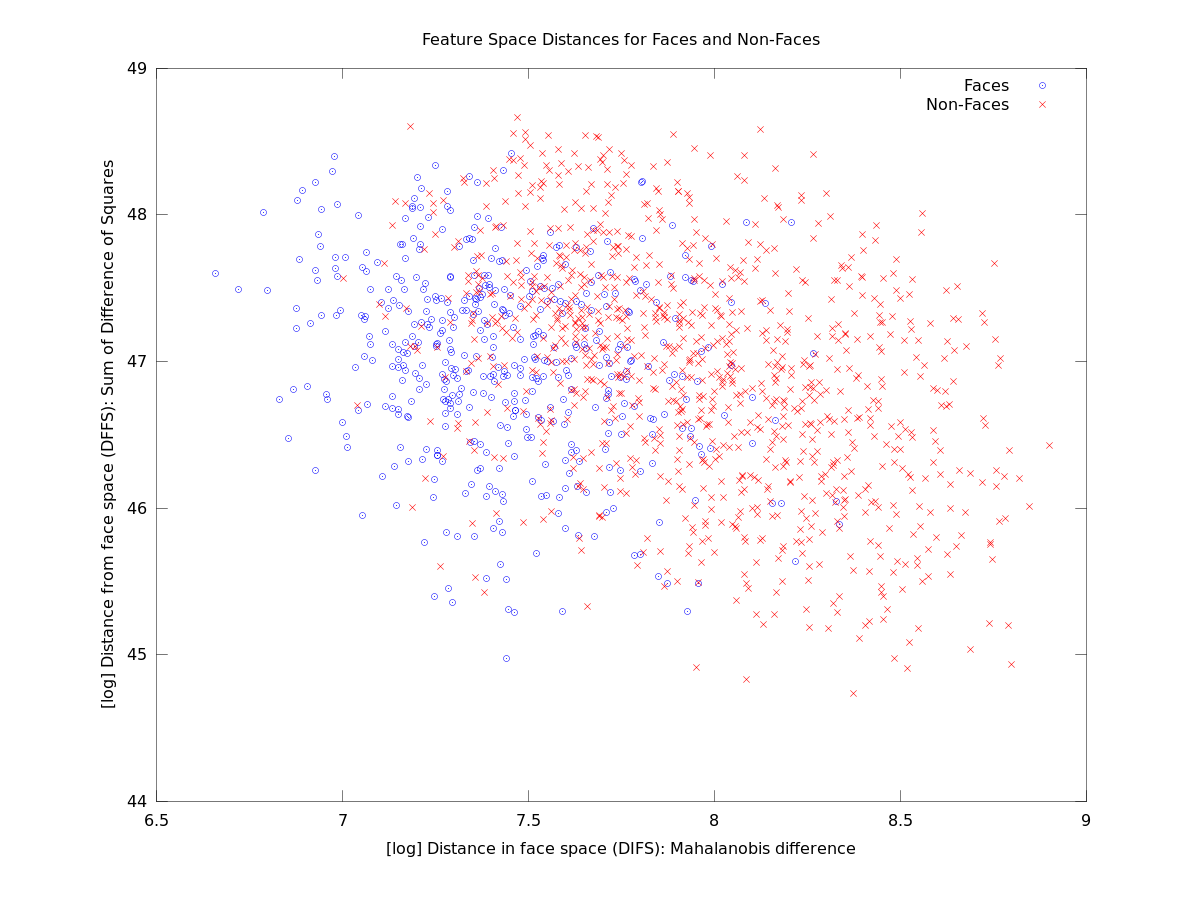
\includegraphics[width=8in]{facespace_distances.png}
    \caption{DIFS and DFFS measures for 1000 faces and 1000 non-faces}
    \label{fig:distances}
\end{figure}

\end{landscape}

The face detection algorithm was implemented in MATLAB as the \verb|pca_face_detect|
function:
 
{\footnotesize
    \verbatiminput{pca_face_detect.m}
}

\subsection{Demonstration}
PCA face detection is demonstrated in MATLAB with the \verb|pca_face_demo| function:

{\footnotesize
    \verbatiminput{pca_face_demo.m}
}


\bibliographystyle{plain}
\bibliography{cap6411_JaimeSoto_hw03}

\end{document}
